% Ustawienia dokumentu
\documentclass[11pt,oneside]{book}
\usepackage[T1]{fontenc}
\usepackage[utf8]{inputenc}
\usepackage{graphicx}
\usepackage{amsmath,amssymb,amsfonts}
\usepackage{txfonts}
\usepackage{listings}
\usepackage[polish]{babel}
\usepackage{fullpage}
\usepackage{color}
\usepackage{caption}
\usepackage[pdftex]{hyperref}

\hypersetup{
  colorlinks,
  urlcolor=blue,
  citecolor=red,
  linkcolor=red
}
\urlstyle{rm}
\linespread{1.2}  % interlinia
\captionsetup[figure]{name=Rys.}

% definicje typów
\definecolor{LightGray}{cmyk}{0,0,0,0.1}
\newtheorem{definition}{Definicja}

% informacje o dokumencie
\author{Paweł~Placzyński}
\title{System aukcyjny w~Ruby~on~Rails}
\date{\today}

% DOKUMENT
\begin{document}

\tableofcontents

\chapter{Wstęp}

\newpage

\section*{Wstęp}
\addcontentsline{toc}{chapter}{Wstęp}

Głównym powodem, dla którego powstała ta~praca jest próba zainteresowania programistów organizacją pracy i~metodologią Scrum. Filozofia ta, w~porównaniu ze~znanymi, prototypowymi modelami procesu powstawania oprogramowania, sprawdza się znacznie lepiej w~niewielkich zespołach projektowych. Znajomość tej metodyki (lub podobnych metodyk Agile) zwiększa szanse małym firmom programistycznym na~zaistnienie na~rynku.


Drugim, równie ważnym, powodem było zaciekawienie czytelnika technologiami i~narzędziami, takimi jak: język \textit{Ruby} oraz aplikacja szkieletowa \textit{Ruby~on~Rails}. Stosowanie tych narzędzi stanowi dobrą alternatywę dla znanych w~dziedzinie technologii, takich jak język \textit{PHP}, \textit{Java} lub \textit{.NET}.


\subsection*{Cele pracy}

Cele, jakie zamierzam osiągnąć pisząc tę~pracę są~następujące:

\begin{itemize}
  \item Przybliżenie metodologii Scrum -- zamierzam zaprezentować działanie metodologii Scrum na~przykładzie procesu tworzenia projektu systemu aukcyjnego;
  \item Opis zastosowania technologii Ruby~on~Rails w~problemie stworzenia systemu aukcyjnego -- przedstawienie procesu tworzenia aplikacji przy pomocy aplikacji szkieletowej Ruby~on~Rails;
\end{itemize}

\subsection*{Problematyka}

Praca dotyczy zagadnień inżynierii oprogramowania. Zasadniczym problemem pracy jest zaprojektowanie oraz~implementacja systemu aukcyjnego przy użyciu aplikacji szkieletowej Ruby~on~Rails.

Zakres pracy obejmuje następujące zagadnienia:

\begin{itemize}
  \item prezentacja języka Ruby oraz~aplikacji szkieletowej Ruby~on~Rails;
  \item zaprojektowanie oraz~implementacja systemu aukcyjnego przy użyciu aplikacji szkieletowej Ruby~on~Rails;
  \item przedstawienie przebiegu pracy nad projektem przy zastosowaniu się do~zasad metodologii Scrum;
\end{itemize}

\subsection*{Struktura pracy}

W~pierwszym rozdziale pracy przybliżono technologie użyte podczas tworzenia systemu aukcyjnego w~Ruby~on~Rails. Rozdział ten opisuje także narzędzia, przy pomocy których powstał ten projekt.


Rozdział drugi przybliża metodykę oraz organizację pracy nad projektem. Opisane zostały tu~konwencje stosowane przez programistów języka Ruby. Ponadto, została zaprezentowana filozofia pracy w~zespołach programistycznych, stosujących programowanie zwinne.


Rozdział trzeci opisuje szczegółowo powstały projekt -- system aukcyjny. Opisany został tu~proces instalacji i konfiguracji środowiska pracy, omówione zostały założenia projektu, przybliżono architekturę oraz przedstawiono historię pracy nad projektem. W~rozdziale tym znajduje się także podręcznik użytkownika, objaśniający istotę działania systemu.


Ostatni rozdział zawiera obserwacje poczynione podczas tworzenia systemu aukcyjnego oraz krótkie podsumowanie pracy nad projektem.


\chapter{Technologie i~narzędzia}

\textit{W~poniższym rozdziale opisane są~technologie oraz~narzędzia, które wykorzystane zostały podczas realizacji systemu aukcyjnego w~Ruby~on~Rails.}

\section{Opis technologii zastosowanych w~pracy}

% język, framework i środowisko testowe

\subsection{Ruby oraz Ruby~on~Rails} \label{technologie.baza}

\subsubsection{Ruby 1.9.3} \label{technologie.ruby}

Ruby (z.~ang.~ruby -- rubin) -- interpretowany, w~pełni obiektowy i~dynamicznie typowany język programowania stworzony w~1995 roku przez Yukihiro Matsumoto (pseudonim Matz). Wersja 1.9.2 cechuje się szybszym interpreterem, mniejszą konsumpcją zasobów oraz drobnymi poprawkami w~standardowych bibliotekach języka.

\subsubsection{Ruby~on~Rails 3.1.0} \label{technologie.ror}

Ruby~on~Rails\footnote{\url{http://rubyonrails.pl/}} (często nazywany RoR lub po~prostu Rails) to~framework open source służący do~szybkiego tworzenia aplikacji webowych stworzony głównie przez duńskiego programistę Davida Heinemeiera Hanssona w~ramach pracy nad oprogramowaniem Basecamp\footnote{Patrz: \url{http://basecamphq.com/}}. Rails to~w~pełni wyposażone środowisko do~tworzenia aplikacji internetowych opartych o~bazy danych zgodnie ze~wzorcem MVC (Model-View-Controller). Ruby~on~Rails daje programiście środowisko w~pełni oparte o~język programowania Ruby -- od~Ajax'a dostępnego w~widokach (View), do~zapytania i~odpowiedzi w~kontrolerach i~logice biznesowej modeli.


Tuż po~pojawieniu się Ruby~on~Rails na~forum publicznym okrzyknięto go~sensacyjnym. Tim O'Reilly, Założyciel O'Reilly Media mówił\footnote{Źródło: \url{http://www.rubyonrails.pl/cytaty}} ,,Ruby on Rails jest przełomem w~dziedzinie programowania aplikacji internetowych. Potężne aplikacje, których tworzenie do~tej pory zabierało tygodnie czy miesiące, są~teraz tworzone dosłownie w~kilka dni.''


Niestety -- w~ciągu ostatnich trzech lat spadło zainteresowanie technologią Ruby~on~Rails (patrz wykres \ref{fig.wykres.googleresearch}). Programiści coraz rzadziej sięgają po~ten produkt wybierając nowsze rozwiązania takie jak Django\footnote{Patrz: \url{http://www.djangoproject.com/}} napisane w~języku Python\footnote{Patrz: \url{www.python.org}}. Nadzieją na~poprawienie tej sytuacji jest nowo wydana -- trzecia wersja frameworku Ruby~on~Rails oraz~ciągły rozwój dodatków -- wtyczek \texttt{gem}. Dlatego też chcę przybliżyć tę~technologię i~zachęcić do~jej używania.

\begin{figure}[!t]
\centering
\includegraphics[width=\textwidth]{obrazki/googleresearch.png}
\caption{Statystyka wyszukiwarki Google na~temat znanych aplikacji szkieletowych (źródło: \url{http://www.google.com/insights/search/\#cat=5\&q=Ruby\%20on\%20Rails\%2CDjango\%2CSpring\%20MVC\&cmpt=q}).}
\label{fig.wykres.googleresearch}
\end{figure}

Liczby na~wykresie \ref{fig.wykres.googleresearch} wskazują, ile wyszukiwań przeprowadzono na~podstawie określonego hasła w~porównaniu do~łącznej liczby wyszukiwań przeprowadzonych w~Google w~tym czasie. Wartości te~nie odzwierciedlają bezwzględnej liczby wyszukiwań, ponieważ dane są~znormalizowane i~przedstawione na~skali od~0 do~100. Każdy punkt na~wykresie jest dzielony przez wartość najwyższego punktu. Jeśli ilość danych jest za~mała, podawana jest wartość 0. Liczby wyświetlane nad wykresem obok wyszukiwanych haseł stanowią podsumowania lub wartości łączne\footnote{Źródło: \url{http://www.google.com/support/insights//bin/answer.py?hl=pl\&answer=87285}}.

\subsubsection{RSpec + Cucumber}

RSpec\footnote{\url{http://rspec.info/}} to~narzędzie do~testownia oprogramowania pod względem testów jednostkowych oraz~behawioralnych przydatne w~realizowaniu projektów Test Driven Developement oraz~Behavior Driven Developement. Narzędzie Cucumber\footnote{\url{http://cukes.info/}} pozwala na~testowanie oprogramowania na podstawie tzw. scenariuszy -- dokumentów napisanych w języku naturalnym opisujących krok po~kroku funkcjonalności projektu.

% gemy, rozszerzenia, pluginy, dodatki, etc.

\subsection{Gemy i pluginy} \label{technologie.gemy}

\begin{enumerate}
  \item \texttt{haml}\footnote{\url{http://haml-lang.com/}} + \texttt{sass}\footnote{\url{http://sass-lang.com/}} -- plugin obsługujący język znaczników HAML używany do~prostego i~przejrzystego opisywania dokumentów XHTML oraz~CSS.
  \item \texttt{device}\footnote{\url{https://github.com/plataformatec/devise}} -- system obsługi autentyfikacji użytkowników (rejestracja, sesje, zarządzanie hasłami itp.).
  \item \texttt{thinking-sphinx}\footnote{\url{http://freelancing-god.github.com/ts/en/}} -- potężny silnik wyszukiwania i~dopasywania danych do podanych wzorców w~relacyjnych bazach danych.
  \item \texttt{will\_paginate}\footnote{\url{https://github.com/mislav/will\_paginate/wiki}} -- plugin obsługujący paginację stron.
  \item \texttt{tiny\_mce}\footnote{\url{http://tinymce.moxiecode.com/}} -- plugin pozwalający na~użycie wewnętrznego edytora HTML.
  \item \texttt{sqlite3}\footnote{\url{http://www.sqlite.org/}} -- adapter bazy danych Sqlite w~wersji trzeciej.
\end{enumerate}

% technologie webowe

\subsection{Technologie W3 i poboczne} \label{technologie.web}

\begin{enumerate}
  \item \texttt{XHTML5}\cite{html5doc} (z~ang.~HyperText Markup Language version 5 -- język znaczników hipertekstu w~wersji piątej). XHTML5 jest językiem określającym strukturę stron internetowych. Składniowo bazuje on~na~języku XML (jest podzbiorem języka XML). Wersja piąta zapewnia kompatybilność wsteczną względem poprzednich wersji, a~przy tym precyzuje niejasności wersji 4 powodujące nieoczekiwane zachowanie w~niektorych przeglądarkach.
  \item \texttt{CSS3}\cite{css3doc} (z~ang.~Cascade Style Sheet version 3 -- kaskadowy arkusz styli w~wersji trzeciej). CSS3 jest językiem określającym wygląd elementów języka XML jaki wyświetlany jest w~przeglądarce. Wersja 3 zapewnia kilka dodatkowych opcji, jak np. grid layouts (szablony pozycjonowane na bazie siatki)\footnote{\url{http://www.w3.org/TR/css3-grid/}}, shadows and rounded borders (cienie obiektów, zaokrąglenia obramowania)\footnote{\url{http://www.w3.org/TR/css3-background/}}, itp.
  \item \texttt{JavaScript} -- jest małym, lekkim, zorientowanym obiektowo wieloplatformowym językiem skryptowym. JavaScript, mimo że nie jest użyteczny jako samodzielny język, został stworzony z myślą o łatwym zagnieżdżaniu w innych produktach i aplikacjach, jak na przykład przeglądarki internetowe. JavaScript może zostać powiązany z wewnętrzną strukturą danego środowiska dając programiście swobodną kontrolę nad jego elementami.

  \item \texttt{AJAX} (z~ang. Asynchronous JavaScript and XML, asynchroniczny JavaScript i~XML) -- technologia tworzenia aplikacji internetowych, w~której interakcja użytkownika z~serwerem odbywa się bez przeładowywania całego dokumentu, w~sposób asynchroniczny. Ma~to~umożliwiać bardziej dynamiczną interakcję z~użytkownikiem niż w~tradycyjnym modelu, w~którym każde żądanie nowych danych wiąże się z~przesłaniem całej strony HTML.

  \item \texttt{jQuery}\footnote{\url{http://docs.jquery.com/Main\_Page}} (z.~ang. query -- zapytanie) -- lekka biblioteka programistyczna dla języka JavaScript, ułatwiająca korzystanie z~JavaScript (w~tym manipulację drzewem DOM). Kosztem niewielkiego spadku wydajności w~stosunku do~profesjonalnie napisanego kodu w~niewspomaganym JavaScripcie pozwala osiągnąć interesujące efekty animacji, dodać dynamiczne zmiany strony, wykonać zapytania AJAX. Większość pluginów i~skryptów opartych o~jQuery działa na~stronach nie wymagając zmian w~kodzie HTML (np.~zamienia klasyczne galerie złożone z~miniatur linkujących do~obrazków w~dynamiczną galerię). Wszystkie efekty osiągnięte z~pomocą jQuery można osiągnąć również bez jej użycia. Jednak kod okazuje się nieporównywalnie dłuższy i~bardziej skomplikowany.
\end{enumerate}


\section{Narzędzia użyte podczas pisania pracy}

\subsection{Kontrola pracy w~Scrum}

\begin{enumerate}
  \item \texttt{git}\footnote{\url{http://git-scm.com/}} -- system kontroli wersji bazujący na~przechowywaniu plików różnic -- tzw. plików diff.
  \item \texttt{tig} narzędzie \texttt{ncurses} służące do~prostego zarządzania repozytorium \texttt{git}
  \item \texttt{ticgit}\footnote{\url{https://github.com/schacon/ticgit/wiki/}} -- issue tracker działajacy jako rozszerzenie dla systemu kontroli wersji git; zapisuje zmiany w~trackingu w oddzielnej gałęzi repozytorium git projektu.
\end{enumerate}

\subsection{Środowisko programistyczne}

\begin{enumerate}
  \item \texttt{zsh + screen}
  \item \texttt{vim}\footnote{\url{http://www.vim.org/}} -- edytor tekstu.
  \item \texttt{RVM}\footnote{\url{https://rvm.beginrescueend.com/}} -- system kontrolii wersji języka Ruby.
  \item \texttt{IRB} -- interaktywna konsola języka Ruby.
  \item \texttt{rspec} + \texttt{cucumber} -- patrz rozdział \ref{technologie.gemy}
  \item \texttt{Sqliteman}\footnote{\url{http://sqliteman.com/}} -- narzędzie do~zarządzania bazami danych Sqlite3.
\end{enumerate}

\subsection{Wdrożenie}

Do~pełnego przedstawienia cyklu pracy nad projektem wykonanym w~technologii Ruby~on~Rails potrzebne jest przedstawienie metod wdrożenia aplikacji webowej oraz~zaproponowanie sposobu jej konserwacji. W~tym celu mam zamiar przybliżyć jedne z~najprostszych znanych mi sposobów wdrożenia aplikacji Ruby~on~Rails.

\begin{enumerate}
  \item \texttt{heroku}\footnote{\url{http://www.heroku.com/}} -- serwis pozwalający na~tworzenie deploymentu projektów napisanych w języku Ruby ,,w~chmurze''.
  \item \texttt{Nginx + thin}\footnote{Nginx: \url{http://wiki.nginx.org/NginxPl}, Thin: \url{http://code.macournoyer.com/thin/}} -- lokalne wdrażanie aplikacji przy użycu serwera HTTP \texttt{Nginx} oraz~lekkiego serwera \texttt{thin}.
\end{enumerate}


\chapter{Metodyka pracy}

\textit{W~tym rozdziale opisana została organizacja pracy nad projektem, konwencje użyte podczas tworzenia aplikacji oraz~standardy pracy w~zespole programistycznym.}

\section{Metodyka Scrum} \label{scrum}

Jednym z~podstawowych celów pracy inżynierskiej jest przedstawienie wykorzystanych w~niej technologii, narzędzi i~metod.


\textit{Scrum} \cite{scrumaliance} (ang. przepychanka, młyn) jest jedną z~wielu pochodnych metodyki programowania zwinnego \cite{agile1} (ang. agile programming).

\subsection{Programowanie zwinne} \label{scrum.agile}

\textit{Programowanie zwinne} jest popularną metodą pracy w~wielu firmach parających się programowaniem. Dla wyjaśnienia czym tak naprawdę jest, wystarczy definicja \cite{agile2}:

\begin{quote}
Programowanie zwinne (ang. agile software development) to~grupa metodyk wytwarzania oprogramowania opartego o~programowanie iteracyjne (model przyrostowy). Wymagania oraz~rozwiązania ewolu\-ują przy współpracy samozarządzalnych zespołów, których celem jest przeprowadzanie procesów wytwarzania oprogramowania. Pojęcie zwinnego programowania zostało zaproponowane w 2001 w~\textit{Agile Manifesto} \cite{agile.manifesto}
[\ldots]


Generalnie metodyka oparta jest o~zdyscyplinowane zarządzanie projektem, które zakłada częste inspekcje wymagań i rozwiązań wraz z~procesami adaptacji (zarówno specyfikacji jak i~oprogramowania). Metodyka ta~najczęściej znajduje zastosowanie w~małych zespołach programistycznych, w~których nie występuje problem komunikacji, przez co~nie trzeba tworzyć rozbudowanej dokumentacji kodu. Kolejne etapy wytwarzania oprogramowania zamknięte są~w~iteracjach, w~których za~każdym razem przeprowadza się testowanie wytworzonego kodu, zebranie wymagań, planowanie rozwiązań itd. Metoda nastawiona jest na~szybkie wytwarzanie oprogramowania wysokiej jakości.
\end{quote}

\subsection{Scrum} \label{scrum.scrum}

Poniżej omówiono metodykę \textit{Scrum}, wykorzystaną podczas realizacji części praktycznej pracy. Metodyka \textit{Scrum} opiera się na~ścisłych iteracjach, w~których realizowane są~założenia projektowe. Każda iteracja zaczyna się tzw. \textit{Sprint~Meeting'iem} (ang. ,,spotkanie w~biegu'') \cite{scrumaliance}

\begin{figure}[!t]
\centering
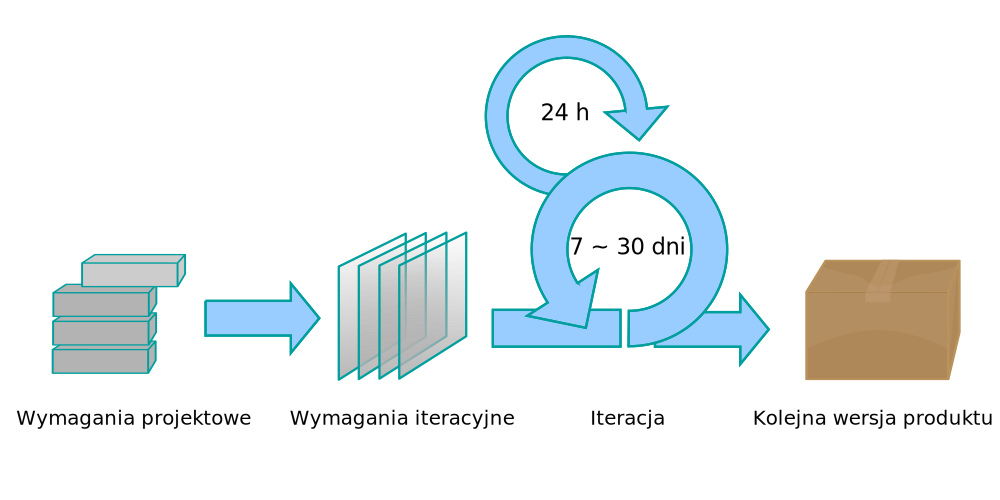
\includegraphics[width=\textwidth]{obrazki/scrum.png}
\caption{Schemat pracy w~kolejnych iteracjach metodyki \textit{Scrum} \cite{scrum.schema}}
\label{fig.rysunek.scrum}
\end{figure}

\subsubsection{Definicje pojęć dla metodyki Scrum} \label{scrum.definicje}

\textit{Iteracją} nazywa się cykl w~procesie wytwarzania oprogramowania, który zamknięty zostaje poprzez zrealizowanie pewnego celu.


Zadania przydzielone zespołowi projektowemu określa się mianem \textit{ticketu}. \textit{Ticket} (ang. bilet) określa jakie obowiązki zostały narzucone na~poszczególnych deweloperów. Jest zwykle odzwierciedleniem żądań i~zaleceń od~klienta.


Główne role jakie można wymienić w~zespole \textit{Scrum} to:

\begin{enumerate}
  \item \textit{Zespół programistyczny} (ang. The Team) -- wykonawcy projektu, deweloperzy w~liczbie do~dziewięciu osób. Do ich obowiązków należy ocena trudności zadań -- \textit{ticketów} -- realizujących założenia projektowe, realizacja tych zadań oraz~zgłaszanie błędów, trudności itp.~zaistniałych w~projekcie.
  \item \textit{Właściciel projektu} (ang. Product Owner) -- jest to~osoba, firma, grupa itp.~będąca zleceniodawcą (klientem) zatrudniającym zespół programistyczny do~zrealizowania projektu. Zasadniczą rolą właściciela projektu jest przedstawianie założeń, wymagań dotyczących~projektu, rewizja wykonanych zadań tegoż zespołu oraz~konsultowanie zmian. Gdy właścicielem projektu jest jakaś większa jednostka (firma, spółka, grupa), wtedy to~wyznaczany jest reprezentant odpowiedzialny za~wyżej wymienione czynności.
  \item \textit{Mistrz młyna} (ang. Scrum Master) -- osoba odpowiedzialna za~komunikację pomiędzy zespołem programistycznym a~właścicielem projektu. Do~jej obowiązków należy przede wszystkim: ustalanie \textit{sprint meeting'ów}, zgłaszanie intencji zespołu programistycznego, wysyłanie powiadomień o~zmianach w~założeniach.
\end{enumerate}

\subsubsection{Rozpoczęcie pracy w~Scrum} \label{scrum.poczatki}

Zanim zostanie rozpoczęta pierwsza iteracja -- \textit{sprint} -- należy dokładnie przemyśleć i~omówić możliwości grupy projektowej oraz~skonfrontować je~z~wymaganiami klienta. W~tym celu organizowane jest spotkanie inicjujące pracę nad projektem. Na~takim spotkaniu powinny zostać omówione następujące kwestie:

\begin{enumerate}
  \item \textit{Metody pracy z~klientem} -- klient powinien wiedzieć jak pracuje zespół czego może się po~nim spodziewać.
  \item \textit{Założenia projektowe} -- zespół programistyczny dowiaduje się jakie są~postawione wobec niego oczekiwania.
  \item \textit{Rewizja założeń projektowych} -- zespół programistyczny ma~szansę wypowiedzieć się na~temat kolejnych założeń i~związanych z~nimi trudności.
  \item \textit{Wycena projektu} oraz~ustalenie licencji jego użytkowania.
\end{enumerate}

Po~omówieniu tych zagadnień klient może zdecydować, czy taki sposób pracy mu~odpowiada. W~tym momencie jest w~stanie oszacować, jak długo będzie współpracował nad projektem z~tą~grupą projektową, a~co~za~tym idzie -- jaką ilość pieniędzy może przeznaczyć na~poszczególnych etapach tworzenia projektu.

\subsubsection{Sprint meeting} \label{scrum.sprintmeeting}

Sprint meeting zamyka jedną iterację i~rozpoczyna następną. Podczas sprint meeting'u realizowane są~następujące działania: sprawdzenie poprawności wykonanych zadań z~poprzedniej iteracji oraz przedyskutowanie planu pracy w następnej iteracji. Pozwala to~klientowi na~pełną kontrolę nad procesem wytwarzania projektu. Do~najważniejszych kwestii omawianych na~\textit{sprint meeting'u} należą:

\begin{enumerate}
  \item Sprawdzenie stanu wykonanych zadań -- jeśli zadania zostały dostarczone klientowi jako wykonane, to~klient może je~zweryfikować pod względem ich poprawności. Każde takie zadanie może zostać zaakceptowane (wtedy oznaczone zostaje jako wykonane) bądź nie. Zadanie odrzucone wymaga poprawki -- klient może zdecydować, co~powinno być w~tej sytuacji wykonane. Jeżeli klient ma~wystarczająco funduszy na~wykonanie poprawek, może zlecić poprawkę, jeśli nie, to~zadanie może zostać ,,zamrożone'' i~czekać na~pieniądze potrzebne do~jego realizacji. Oczywiście klient może także zaniechać realizacji zadania.
  \item Określenie wymagań projektowych -- klient wymienia swoje oczekiwania względem projektu. Wymagania te~zostają skonfrontowane z~możliwościami zespołu programistycznego (,,tego nie da~się zrobić'', ,,to~jest za~trudne'', ,,to~wymaga lepszego sprzętu'', ,,realizacja tego zadania zajmie \ldots'', ,,koszta tego zadania wyniosą około \ldots'', albo: ,,to~jest proste'', ,,znamy się na~tym''). Zwykle zaistniałe trudności w~realizacji zadań kończą się kompromisem. Po~określeniu możliwości realizacji wymagań tworzone są~zadania.
  \item Określenie zadań dla grupy projektowej -- po~,,wycenie'' możliwości deweloperów względem wymagań tworzone są~zadania. Zwykle rozbija się je~na~prostsze, wymagające mniej czasu (według zasady ,,dziel i~zdobywaj'') -- uzyskuje się wtedy płynność w~realizacji zadań, a~praca nad konkretnym wymaganiem podzielona jest pomiędzy członków zespołu.
  \item Przydzielenie zadań -- klient po~określeniu i~sprecyzowaniu zadań określa ich priorytet. Niektóre zadania są~ważniejsze -- te~oznaczane są~jako zadania przypisane nadchodzącej iteracji -- nad tymi zadaniami grupa projektowa będzie w~najbliższym czasie pracować. Zadania te~zostają następnie wybierane przez konkretnych deweloperów jako te, które będą przez nich realizowane. Jeżeli po~zakończonej iteracji zostaną zadania niewykonane przez nikogo, to oznacza to, że~grupa nie nadąża z~tempem pracy narzuconym przez klienta.
  \item Ustalenie ,,dostępności'' deweloperów w~najbliższej iteracji -- członkowie zespołu mogą z~różnych powodów nie móc pracować w~pewnym okresie czasu. Z~tego względu pod koniec sprint meeting'u należy ustalić ile godzin pracy każdy deweloper może przeznaczyć na~najbliższą iterację. Pozwala to~określić ,,siłę'' zespołu oraz~długość iteracji. W~szczególnych przypadkach iteracje mogą zostać przeniesione bądź zawieszone ,,do~odwołania''.
\end{enumerate}

\subsection{Narzędzia Scrum} \label{scrum.narzedzia}

Narzędzi, które wspomagają pracę w~metodyce Scrum jest wiele. Przykładem mogą być tzw. \textit{Issue Tracker'y} -- środowiska do~zarządzania ticketami. Dobrym przykładem takiego \textit{Issue Trackera} jest \textit{PivotalTracker}\footnote{\url{www.pivotaltracker.com}}. Pozwala on~na~kontrolowanie zadaniami poprzez oznaczanie ich jako wykonanych, bieżących itp. Przykładowe zastosowanie tego narzędzia w~pracy nad projektem przedstawia rysunek \ref{fig.rysunek.pivotal}.

\begin{figure}[!t]
\centering
\includegraphics[width=\textwidth]{obrazki/pivotal.png}
\caption{Zastosowanie narzędzia \textit{PivotalTracker} w~pracy nad projektem. \cite{pivotaltracker}}
\label{fig.rysunek.pivotal}
\end{figure}

Innym przykładem narzędzia wspomagającego pracę w~projekcie \textit{Scrum} są~testy jednostkowe i~funkcjonalne aplikacji (patrz rozdział \ref{dokumentacja.testy}). Służą one tutaj przede wszystkim rewizji zaimplementowanej funkcjonalności a zatem sprawdzeniu poprawności wykonania zadania. Testy takie są~zatem udokumentowaniem wykonanej pracy przez dewelopera.


\section{Dokumentacja projektu} \label{dokumentacja}

Projekty systemów informatycznych mają to~do~siebie, że~rozwijają się niezwykle szybko. Rozwój projektu związany jest niestety z~powiększaniem objętości projektu -- zarówno merytorycznej, jak i~czysto fizycznej (ilość linijek kodu, ilość plików). Problem pojawia się, gdy projekt jest zbyt ,,duży'' żeby programista mógł rozumieć wszystko to, co~się w~nim dzieje. Rozwiązaniem dla tego problemu jest tworzenie dokumentacji.


W~projektach typu \textit{OpenSource} dokumentacja jest niezwykle ważnym czynnikiem usprawniającym pracę programistów w~nich pracujących. Dobrze napisana dokumentacja sprawia, że~nowe osoby zaczynające pracę w~projekcie mogą łatwiej i~szybciej zapoznać się ze~strukturą, działaniem oraz~organizacją projektu. Jest to~szczególnie przydatne, gdy istnieje potrzeba edycji jedynie niewielkiego fragmentu projektu. Co~więcej -- osoby zajmujące się już od~dłuższego czasu pracą w~takim projekcie nie muszą pamiętać wszelkich zagadnień z~nim związanych.


\subsection{Kod aplikacji} \label{dokumentacja.kod}

Najlepszą dokumentacją dla systemu informatycznego jest kod aplikacji. To~właśnie on~realizuje wszystkie założenia projektowe, algorytmy lub cykle pracy projektu. Prawidłowo napisany kod może powiedzieć więcej niż nie jedna dokumentacja -- tu~dowiadujemy się, jak naprawdę działa interesujący nas moduł i~mamy pewność, że~nie padniemy ofiarą nieporozumień. Pod pojęciem ,,prawidłowo napisany kod'' rozumie się spełnienie następujących założeń:

\begin{itemize}
  \item trzymanie się konwencji określającej osnowę dokumentu, zawierającego kod,
  \item stosowanie zrozumiałych nazw dla wszelkich struktur (nazwy klas, metod, zmiennych),
  \item tworzenie krótkich i~treściwych fragmentów kodu oraz~rozbijanie większych partii na~mniejsze.
\end{itemize}

Wszystkie te kroki mają na celu sprawienie, że~kod stanie się bardziej czytelny. Poniżej omówiono te~trzy kroki nieco dokładniej w~zastosowaniu dla języka Ruby.

\subsubsection{Konwencja} \label{dokumentacja.konwencja}

Język Ruby ze~względu na~swoją składnię jest niezwykle czytelny, a~co~za~tym idzie, kod w~nim napisany jest łatwy w~zrozumieniu. Składnia Rubiego przypomina pseudokod:

  \lstset{language=Ruby, caption=Przykład prostej składni języka Ruby -- algorytm DFS., basicstyle=\ttfamily\footnotesize, numbers=left, numberstyle=\footnotesize, captionpos=b, backgroundcolor=\color{LightGray}} \label{code.simpleruby}
  \begin{lstlisting}
  def dfs node, value, queue
    return false if node.nil?
    return true if node.data == value
    queue.push node.right_neighbor unless node.right_neighbor.nil?
    queue.push node.left_neighbor unless node.left_neighbor.nil?
    dfs queue.pop, value, queue
  end
  \end{lstlisting}

Niestety -- sama składnia nie jest najważniejsza w~dokumentowaniu projektów. Powyższy przykład można przecież przepisać w~inny sposób:

  \lstset{language=Ruby, caption=Algorytm DFS z~zastosowaniem braku konwencji formatu., basicstyle=\ttfamily\footnotesize, numbers=left, numberstyle=\footnotesize, captionpos=b, backgroundcolor=\color{LightGray}}
  \begin{lstlisting}
  def dfs node, value, queue
  return false if node.nil?; if node.data == value
  return true
  end; queue.push node.right_neighbor unless \\
    node.right_neighbor.nil?
  unless node.left_neighbor.nil?
  queue.push node.left_neighbor; end
  dfs queue.pop, value, queue
  end
  \end{lstlisting}

Przykład ten jest mniej czytelny, a~co~za~tym idzie, trudniej jest dowiedzieć się, za~co~dany fragment kodu jest odpowiedzialny. W~celu uzyskania ,,przejrzystości'' kodu stosuje się konwencje zapisu -- ogólnie przyjęte zasady mówiące o~tym jak powinien wyglądać kod i~jak ten kod formatować. Język Ruby posiada swoją konwencję o~nazwie \textit{The Ruby Style} \cite{therubyway}, która określona jest następująco:

\begin{enumerate}
  \item Formatowanie:
  \begin{enumerate}
    \item Używaj zawsze kodowania ASCII lub UTF8.
    \item Używaj dwóch spacji jako wcięć (nigdy tabulatur).
    \item Staraj się kończyć wiersz w~stylu używanym w~systemach Unix (LF -- 0x0A).
    \item Używaj spacji przed i~po~operatorach, po~przecinkach, po~dwukropkach, po~średnikach, przed i~po~\{ oraz~po~\}.
    \item Nie używaj spacji po~( oraz~[. Nie używaj spacji przed~] oraz~).
    \item Używaj dwóch spacji przed modyfikatorem warunku (\texttt{if}/\texttt{unless}/\texttt{while}/\texttt{until}/\texttt{resque}).
    \item Wcięcie dla słowa kluczowego \texttt{when} powinno być tak głębokie, jak dla \texttt{case}.
    \item Użyj pustego wiersza przed zwracaną wartością w~metodzie (chyba, że~ma~ona tylko jeden wiersz), a~także przed słowem kluczowym \texttt{def}
    \item Używaj RDoc do~dokumentacji API. Nie wstawiaj pustego wiersza pomiędzy komentarz a~komentowany blok.
    \item Użyj pustego wiersza do~podzielenia dużych metod na~logiczne fragmenty.
    \item Staraj się, aby~każdy wiersz miał mniej niż 80 znaków.
    \item Unikaj białych znaków na~końcu wiersza.
  \end{enumerate}
  \item Składnia:
  \begin{enumerate}
    \item Użyj \texttt{def} z~ nawiasami, gdy są~podane argumenty.
    \item Nie używaj \texttt{for}, chyba, że~robisz to~celowo.
    \item Nie używaj \texttt{then}.
    \item Użyj ,,\texttt{when x;} \ldots'' dla jednolinijkowego wyrażenia \texttt{case}.
    \item Użyj \texttt{\&\&}/\texttt{||} dla wyrażeń boolowskich, \texttt{and}/\texttt{or} do~kontroli przepływu.
    \item Unikaj wielolinikowej instrukcji \texttt{?:}, użyj \texttt{if}.
    \item Zaniechaj użycia nawiasów przy wywołaniu metod, ale użyj ich podczas wywołania ,,funkcji'' (na~przykład~gdy używasz zwracanej wartości w~tym samym wierszu)
    \item Używaj raczej \mbox{\texttt{\{} \ldots \texttt{\}}} niż \mbox{\texttt{do} \ldots \texttt{end}}. Wielolinijkowe bloki \mbox{\texttt{\{} \ldots \texttt{\}}} są~w~porządku: używając \texttt{\}} na końcu bloku wiemy, że~kończy się blok a~nie instrukcja \texttt{if}/\texttt{while}/\ldots. Używaj \mbox{\texttt{do} \ldots \texttt{end}} do~kontroli przepływu (na~przykład~zadania \texttt{rake}, bloki \texttt{sinatra}).
    \item Unikaj używania słowa kluczowego \texttt{return} jeśli nie jest potrzebne.
    \item Unikaj kontynuacji linii (\texttt{$ \backslash $}) jeśli nie musisz.
    \item Używanie zwracanej wartości przez operator \texttt{=} jest na miejscu.
    \item Używaj operatora \texttt{||=}.
    \item Używaj wyrażeń regularnych typu ,,non-OO''.  Nie bój się używać \texttt{=~}, \texttt{\$0-9}, \texttt{\$~}, \texttt{\$`} oraz~\texttt{\$'} jeśli potrzebujesz.
  \end{enumerate}
  \item Nazewnictwo:
  \begin{enumerate}
    \item Używaj \textit{snake\_case} jako stylu nazywania metod.
    \item Używaj \textit{CamelCase} jako stylu nazywania klas i~modułów (pozostaw akronimy takie jak HTTP, RFC, XML z~wielkich liter).
    \item Używaj SCREAMING\_SNAKE\_CASE jako stylu nazywania stałych.
    \item Długość nazwy zwykle określa kontekst wykorzystania. Używaj jednoliterowych zmiennych jako parametrów bloków/metod według tego schematu:\\
      \texttt{a}, \texttt{b}, \texttt{c}, \texttt{o}: dowolny obiekt;\\
      \texttt{d}: katalog;\\
      \texttt{e}: element (klasy Emumerable oraz~pochodnych);\\
      \texttt{ex}: wyjątek;\\
      \texttt{f}: plik:\\
      \texttt{i}, \texttt{j}: indeksy;\\
      \texttt{k}: klucz tablicy asocjacyjnej;\\
      \texttt{m}: metoda;\\
      \texttt{r}: zwracana wartość krótkich metod;\\
      \texttt{s}: tekst;\\
      \texttt{v}: wartość elementu tablicy asocjacyjnej;\\
      \texttt{x}, \texttt{y}, \texttt{z}: liczby;\\
      Ponadto, pierwsza litera klasy obiektu może posłużyć za~nazwę takiej zmiennej.

    \item Używaj nazw zaczynających się od~\texttt{\_} dla nieużywanych zmiennych.
    \item Używając \texttt{inject} dla krótkich bloków nazywaj argumenty \texttt{|a, e|} (od:~akumulator, element).
    \item Definiując operatory dwuargumentowe, nazywaj argument jako ,,other''.
    \item Używaj raczej \texttt{map} niż \texttt{collect}, \texttt{find} niż \texttt{detect}, \texttt{find\_all} niż \texttt{select} oraz~\texttt{size} niż \texttt{length}.
  \end{enumerate}
  \item Komentarze:
  \begin{enumerate}
    \item Komentarze dłuższe niż słowo rozpoczynają się z~wielkiej litery i~używane są zasady interpunkcji.
    \item Używaj dwóch spacji po każdej kropce w komentarzu.
    \item Unikaj niepotrzebnych komentarzy.
  \end{enumerate}
  \item Pozostałe:
  \begin{enumerate}
    \item Pisz kod przyjazny dla opcji \texttt{ruby -w}.
    \item Unikaj tablic asocjacyjnych jako opcjonalnych parametrów.
    \item Unikaj długich metod.
    \item Unikaj długich list parametrów.
    \item Używaj konstrukcji \texttt{def self.}\textit{metoda} dla zdefiniowania metod singletonów.
    \item Staraj się rozwijać funkcjonalność standardowych metod.
    \item Unikaj \texttt{alias} -- używaj \texttt{alias\_method}.
    \item Używaj \texttt{OptionParser} do~parsowania skomplikowanych opcji wejścia konsoli a~\texttt{ruby -s} dla rozwiązań trywialnych.
    \item Staraj się zachować zgodność wielu wersji interpretera.
    \item Unikaj zbędnego metaprogramowania.
  \end{enumerate}
  \item Ogólne zasady:
  \begin{enumerate}
    \item Programuj w sposób funkcjonalny.
    \item Nie wydziwiaj z~używaniem argumentów metod -- chyba, że~wiesz co robisz.
    \item Nie zmieniaj funkcjonalności standardowych bibliotek pisząc własne.
    \item Nie programuj zachowawczo\footnote{Patrz: \url{http://www.erlang.se/doc/programming\_rules.shtml\#HDR11}}.
    \item Postaraj się zachować prostotę kodu.
    \item Nie przesadź z~projektowaniem.
    \item Ale także nie pozostaw swojej pracy niezaprojektowanej.
    \item Unikaj błędów.
    \item Poczytaj o innych konwencjach, aby móc rozwinąć tę.
    \item Bądź konsekwentny.
    \item Używaj prostych rozwiązań.
  \end{enumerate}
\end{enumerate}

Stosowanie tej konwencji zapewni, że~kod napisany przez nas będzie zgodny z~ogólnym standardem.

\subsubsection{Nazewnictwo w~kodzie} \label{dokumentacja.nazewnictwo}

Aby zrozumieć istotę działania projektu należy zrozumieć mechanizmy i~algorytmy rządzące jego logiką. Zakładając, że~chcemy dobrze odokumentować projekt, trzeba tak napisać kod, by~był zrozumiały -- jak pseudokod opisujący algorytm. W~tym celu wystarczy, że~wszelkie obiekty w~ kodzie, nazwiemy tak, by~ich użycie w~kontekscie było zrozumiałe a~ich rola jasna. W~trakcie pisania kodu najtrudniejszą kwestią jest nazywanie obiektów, a~nie -- jak to~się powszechnie uznaje -- rozwiązanie logiki systemu.

\subsection{Komentarze} \label{dokumentacja.komentarze}

Komentarze w~kodzie to~dobrzy sposób na~wyjaśnienie zasadności użycia algorytmów, bądź struktury API poszczególnych elementów kodu. Stosowanie komentarzy pozwala także wyróżnić, co~ważniejsze dla ,,czytelnika'' elementy kodu.

\subsubsection{RDoc} \label{dokumentacja.rdoc}

Istnieje wiele konwencji dotyczących~formy komentarzy. Format komentarzy ma~znaczenie nie tylko podczas czytania kodu -- może on~posłużyć pośrednio do~wygenerowania pełnej dokumentacji API przy użyciu odpowiednich narzędzi.


Komentarze w~języku Ruby mogą być dwojakiego formatu:

  \lstset{language=Ruby, caption=Komentarze w~języku Ruby., basicstyle=\ttfamily\footnotesize, numbers=left, numberstyle=\footnotesize, captionpos=b, backgroundcolor=\color{LightGray}}
  \begin{lstlisting}
    # Komentarz jednolinijkowy rozpoczyna sie
    # od znaku krzyzyka.

    =begin
      Blok komentarza.
      Taki blok rozpoczyna sie od znacznika "=begin"
      a konczy na znaczniku "=end".
      Komentarze jednolinijkowe sa jednak czesciej
      uzywane.
    =end
  \end{lstlisting}


Narzędzie \textit{RDoc}\footnote{Patrz: \url{rdoc.sourceforge.net}} to~narzędzie konsolowe generujące dokumentację API w~zadanym formacie (standardowo jest to~HTML) na~podstawie kodu oraz~komentarzy w~nim zawartych. Aby wygenerować taką dokumentację wystarczy wpisać w~konsoli:

\mbox{\texttt{\$ rdoc <opcje> [plik...] }}

\textit{RDoc} wygeneruje czytelną dokumentację nawet bez komentarzy w~kodzie.

\subsection{Testy} \label{dokumentacja.testy}

Testy to~dodatkowe aplikacje sprawdzające poprawność logiki projektu. Zasadniczą ich funkcją jest dowiedzenie, że~dana funkcjonalność została zaimplementowana poprawnie.


Testować w~aplikacji można wszystko, jednak dobrze jest ustalić co~chce się uzyskać poprzez napisanie testów. Biorąc pod uwagę powyższe kryterium testy dzieli się na:

\begin{enumerate}
 \item \textit{testy jednostkowe} -- sprawdzają poprawność modułów ,,silnika'' aplikacji. Za~pomocą testów jednostkowych testuje się zwykle klasy, metody, stany maszyny, poprawność algorytmów, wejścia i~wyjścia strumieni itp.
 \item \textit{testy behawioralne} -- odpowiadają na~pytanie: ,,co~się stanie, gdy zrobimy \ldots''. Testują one zachowanie aplikacji -- reakcję na~żądania, efekty działania zdarzeń (takich jak, na przykład, wypełnienie formularza).
\end{enumerate}

\subsubsection{Testy jednostkowe RSpec} \label{dokumentacja.rspec}

\textit{RSpec}\footnote{Patrz: \url{rspec.info}} jest narzędziem do~tworzenia testów jednostkowych dla aplikacji napisanych w~języku Ruby. Jego składnia jest prosta, a~testy w~nim napisane -- czytelne:

  \lstset{language=Ruby, caption=Test RSpec testujący klasę \texttt{Array}., basicstyle=\ttfamily\footnotesize, numbers=left, numberstyle=\footnotesize, captionpos=b, backgroundcolor=\color{LightGray}} \label{code.prostytest}
  \begin{lstlisting}
  describe Array do
    describe "#push" do
      it "puts a value at the end of array" do
        array = Array.new
        value = "Some value"
        array.push value
        array.last.should == value
      end
    end
  end
  \end{lstlisting}

W~pierwszej kolejności podaje się opis testu -- krótką informację o~tym co~testujemy i~jakie są oczekiwania względem testowanego obiektu. Wewnątrz bloku testu realizuje się przypadek użycia obiektu. W~każdym momencie można sprawdzić, czy interesujący nas stan obiektu jest zgodny z~naszymi oczekiwaniami. W~tym celu używa się metod \texttt{should} oraz~\texttt{should\_not}.


Testy uruchamiamy podając w~konsoli polecenie \texttt{rspec} oraz~plik z~napisanymi testami:

\mbox{\texttt{\$ rspec nazwa\_pliku\_testu.rb}}

Trzeba pamiętać, że~testy powinny mieć dostęp do~logiki projektu -- na~przykład~poprzez użycie instrukcji \texttt{require}. Efektem działania testu z~przykładu \ref{code.prostytest} będzie:

  \lstset{language=bash, caption=Efekt uruchomienia testu jednostkowego z~poprzedniego przykładu., basicstyle=\ttfamily\footnotesize, numbers=left, numberstyle=\footnotesize, captionpos=b, backgroundcolor=\color{LightGray}}
  \begin{lstlisting}
.

Finished in 0.00258 seconds
1 example, 0 failures
  \end{lstlisting}

Aby zrozumieć, co~stało się podczas testowania, można zmienić format wyjścia na~bardziej przyjazny:

  \lstset{language=bash, caption=Efekt uruchomienia testu jednostkowego z~opcją \texttt{----format d}., basicstyle=\ttfamily\footnotesize, numbers=left, numberstyle=\footnotesize, captionpos=b, backgroundcolor=\color{LightGray}}
  \begin{lstlisting}
Array
  #push
    puts a value at the end of array

Finished in 0.0029 seconds
1 example, 0 failures
\end{lstlisting}

Jak widać \texttt{rspec} poinformował o~tym, które testy ,,przeszły'' -- czyli, które z~testowanych przez funkcjonalności spełniły oczekiwania.

\subsubsection{RSpec jako dokumentacja}

Przykład \ref{code.prostytest} mówi dość dużo o~sposobie użycia elementów logiki projektu. Testy jednostkowe są~tak naprawdę przypadkami użycia tychże elementów. Co~więcej -- przypadki te~realizują się zgodnie z~założeniami twórcy takiego projektu (uruchomione testy ,,przechodzą''). Oznacza to, że~są one dobrą dokumentacją działania i~sposobu użycia poszczególnych obiektów logiki projektu.

\subsubsection{Dokumentacja poprzez testy behawioralne} \label{dokumentacja.cucumber}

Skoro testy jednostkowe są~swego rodzaju dokumentacją, to~także testy behawioralne mogą nią być. Oczywiście ze~względu na~inny cel testy behawioralne będą dokumentować projekt z~innej perspektywy. Testy te~określają zachowanie aplikacji, a~zatem kwestii ściśle związanej z~użytkowaniem. W~praktyce testy behawioralne są~stosowane dla określenia wymagań ze~strony klienta -- zleceniodawcy projektu.


Istnieje kilka narzędzi, przy pomocy których można napisać i~przeprowadzić testy behawioralne. Można do~tego użyć \texttt{rspec} oraz~\texttt{Test::Unit} (czyli narzędzi wykorzystywanych przy pisaniu testów jednostkowych). Dla dobrej czytelności oraz~eleganckiego formatu użyto narzędzia \textit{Cucumber}\footnote{Patrz: \url{cukes.info}}.


\textit{Opisane powyżej metody pracy z~projektem zostały zastosowane w~systemie aukcyjnym, będącym celem pracy.\\\\W~następnym rozdziale zaprezentowany zostanie proces tworzenia systemu aukcyjnego oraz~opisany zostanie utworzony prototyp.}

\chapter{Projekt systemu aukcyjnego}

\textit{W~rozdziale tym opisany został proces tworzenia aplikacji \texttt{auctioneer}, a~także końcowy efekt i~wnioski dotyczące stworzonego systemu aukcyjnego.}

\section{Wprowadzenie}

\subsubsection{Opis zastosowania technologii Ruby~on~Rails w~problemie stworzenia systemu aukcyjnego}

Technologia Ruby~on~Rails umożliwia proste tworzenie aplikacji webowych dowolnego typu. Dla zaprezentowania jej możliwości wybrano system aukcyjny jako przykład aplikacji webowej stworzonej w~tym środowisku. Wybór ten nie jest przypadkowy -- do~tej pory nie opublikowano podobnego systemu aukcyjnego napisanego przy użyciu aplikacji szkieletowej Ruby~on~Rails\footnote{Jedynym możliwym gotowym rozwiązaniem dla wykorzystania aplikacji webowej w~celu wystawiania aukcji/prowadzenia licytacji jest zastosowanie wtyczki \textit{SpreeQuickAuction} (\url{https://github.com/pronix/spree-quick-auction}) dla systemu CMS Spree (\url{https://github.com/pronix/spree-quick-auction}) napisanego w~Ruby~on~Rails.}.


Pomysł jednak nie jest nowatorski -- w~sieci oraz~w~wielu pozycjach książkowych znajdują się przykłady wykonania sklepów internetowych, które są~w~budowie bardzo podobne do~systemów aukcyjnych.


System aukcyjny to~niezwykle rozwlekły i~obszerny temat. Projekt tego typu zatem może być bardzo rozbudowany. Właśnie z~tego względu założono, że~projekt nie będzie ,,dokończony''. Celem nie jest tu~wykonanie pełnego projektu ,,od~początku do~końca'' a~jedynie prezentacja możliwości jakie oferuje Ruby~on~Rails.

\subsubsection{Przedstawienie prototypu systemu aukcyjnego}

Wraz ze~stworzeniem prototypu systemu aukcyjnego zaprezentowano podstawowe rozwią\-zania dla tego rodzaju problemu. Zagadnienie stworzenia systemu aukcyjnego jest problemem typowym dla dziedziny inżynierii oprogramowania. Wymaga wybrania i~opracowania rozwiązań technicznych i~technologicznych oraz~określenia metodyki pracy nad danym zagadnieniem.


Stworzony prototyp jest swego rodzaju prezentacją zastosowanych w~nim technologii oraz~przykładowych rozwiązań.


\section{Przebieg pracy}

W~tym podrozdziale opiszę fazy tworzenia projektu i~jego rozwoju.

\subsection{Przygotowanie środowiska pracy}

Pierwszym krokiem do~stworzenia systemu aukcyjnego w~technologii Ruby~on~Rails jest przygotowanie środowiska, w~którym projekt bedzie tworzony. Pominięto tutaj proces instalacji systemu operacyjnego.

\subsubsection{Instalacja narzędzi}

Większość narzędzi wymienionych w~rozdziale \ref{narzedzia} Narzędzia można zainstalować wpisując w~konsoli następujące polecenie:


\texttt{sudo apt-get install zsh screen ack-grep vim ruby git git-core tig ticgit ticgitweb sqlite3 sqlite3-dev sqliteman curl}


(Polecenie to~zadziała na~Ubuntu~11.10 oraz na~Debianie~Squeeze. Na~innych dystrybucjach zamiast \texttt{apt-get} należy użyć innego manadżera pakietów dostępnego dla danej dystrybucji. Oczywiście nazwy pakietów także mogą się różnić)

\subsubsection{Zarządzanie wersją Ruby -- RVM}

W~celu zainstalowania \textit{RVM} należy wpisać w~konsoli:


\texttt{bash -s stable < <(curl -s https://raw.github.com/wayneeseguin/rvm/master/binscripts/rvm-installer)}


Aby zainstalować Ruby w~wersji 1.9.3 należy wpisać:


\texttt{rvm install 1.9.3}


Po~konfiguracji i~kompilacji zadanej wersji Ruby należy tylko przełączyć się na~nią:


\texttt{rvm --default use 1.9.3}


Polecenie \texttt{ruby -v} powinno wypisać \texttt{ruby 1.ruby9.ruby93p0 (2011-10-30 revision 33570) [x86\_64-linux]}.

\subsubsection{Instalacja Ruby~on~Rails oraz niezbędnych wtyczek}

Ruby~on~Rails instalujemy wpisując:


\texttt{gem install rails}


W~ten sposób można już utworzyć pierwszy, podstawowy projekt Ruby~on~Rails:


\texttt{rails new auctioneer}


Polecenie to~utworzy katalog auctioneer zawierający podstawowe elementy każdego projektu Ruby~on~Rails.

\lstset{language=bash, caption=Zawartość katalogu \textit{auctioneer}, basicstyle=\ttfamily\footnotesize, captionpos=b, backgroundcolor=\color{LightGray}} \label{code.railsdir}
\begin{lstlisting}
app
app/models
app/views
app/views/layouts
app/controllers
app/helpers
app/assets
app/assets/stylesheets
app/assets/javascripts
app/assets/images
app/mailers
script
vendor
vendor/plugins
vendor/assets
vendor/assets/stylesheets
db
config
config/environments
config/locales
config/initializers
log
public
doc
test
test/integration
test/fixtures
test/functional
test/unit
test/performance
tmp
tmp/cache
tmp/cache/assets
lib
lib/tasks
lib/assets
\end{lstlisting}

Aby zainstalować konieczne do~dalszego działania wtyczki należy wyedytować plik \texttt{Gemfile} dopisując linijki z~nazwami oraz numerami wersji wtyczek.

\lstset{language=ruby, caption=Plik \texttt{Gemfile} projektu \textit{auctioneer}., basicstyle=\ttfamily\footnotesize, numbers=left, numberstyle=\footnotesize, captionpos=b, backgroundcolor=\color{LightGray}} \label{code.railsdir}
\begin{lstlisting}
source 'http://rubygems.org'

gem 'rails', '>=3.1.0'
gem 'sqlite3'

gem 'jquery-rails'
gem 'devise'
gem 'haml'
gem 'haml-rails'
gem 'formtastic'
gem 'thin'
gem 'will_paginate'
gem 'wirble', require: nil
gem 'ruby-debug19', require: nil
gem 'rspec-rails', '>= 2.6.1', group: [:development, :test]
gem 'heroku'
gem 'state_machine'

group :assets do
  gem 'sass-rails', "  ~> 3.1.0"
  gem 'coffee-rails', "~> 3.1.0"
  gem 'uglifier', '>= 1.0.3'
  gem 'therubyracer'
end

group :test do
  gem 'factory_girl_rails', '>= 1.1.0'
  gem 'cucumber-rails', '>= 1.0.2'
  gem 'capybara', '>= 1.0.1'
  gem 'database_cleaner', '>= 0.6.7'
  gem 'launchy', '>= 2.0.5'
  gem 'ruby-debug19'
  gem 'email_spec'
end
\end{lstlisting}

Po~edycji pliku \texttt{Gemfile} należy wywołać polecenie \texttt{bundle install}. Wszystkie zależności związane z~wymaganymi wtyczkami zostaną zainstalowane, a~każda zmiana w~pliku \texttt{Gemfile} wymaga ponownego uruchomienia komendy \texttt{bundle install}.

\subsubsection{Kontrola wersji Git}

W~katalogu projektu stworzonego w~poprzednim punkcie należy zainicjować system kontrolii wersji wpisując polecenie:


\texttt{git init}


W~katalogu powstanie podkatalog \texttt{.git} zawierajacy wszystkie niezbędne informacje o historii tworzonego projektu.


W~projekcie mogą znajdować się pliki, dla~których nie chcemy przechowywać historii. Mogą to~być na~przykład pliki tymczasowe, logi, pliki backup, itp. Aby uniknąć dodawania ich do~historii rozwoju projektu należy utworzyć plik \texttt{.gitignore} i~dopisać tam niechciane pliki.


Aby zapisać bieżący stan projektu w~historii należy zaznaczyć zmiany przy pomocy polecenia \texttt{git add .} oraz wykonać commit przy pomocy \texttt{git commit}. Otworzy się domyślny edytor tekstu, w którym należy podać komentarz dotyczący zmian.

\lstset{language=bash, caption=Plik \texttt{.gitignore} projektu \textit{auctioneer}., basicstyle=\ttfamily\footnotesize, captionpos=b, backgroundcolor=\color{LightGray}} \label{code.railsdir}
\begin{lstlisting}
.sass-cache/
vendor/ruby
*~
*.swp
*.swo
tags
log/*
tmp/*
lib/mysql.rb
config/*.yml
[a-zA-Z0-9\.-_]*~
misc
capybara*
coverage
config/*.sphinx.conf
config/environments/dev_local.rb
db/sphinx/*
public/system/*
public/sitemaps/*
backup
nbproject/*
features_report.html
public/services/
public/stylesheets/all.css
public/javascripts/all.js
rerun.txt
mkmf.log
.bundle/
nohup.out
*.sqlite3
.rvmrc
doc/praca_inzynierska.pdf
\end{lstlisting}

\subsubsection{Dalsza konfiguracja}

W~poprzednich krokach została przedstawiona instalacja środowiska programistycznego dla projektu napisanego w~technologii Ruby~on~Rails. Środowisko takie jest już wystarczające i można zacząć właściwą pracę nad projektem, jednakże każde z~wyżej wymienionych narzędzi można skonfigurować według własnego uznania edytując pliki konfiguracyjne.


Do~tworzenia projektu \textit{auctioneer} użyto konfiguracji dostępnej w~repozytorium GitHub: \url{https://github.com/placek/dotfiles}.


Aby zatwierdzić taką instalację należy wykonać następujące polecenie:


\texttt{git clone git://github.com/placek/dotfiles.git; cp dotfiles/* ~}

\subsection{Założenia projektu}

Zanim programista przystępuje do~pracy należy wyznaczyć szczegółowo zadania i~założenia. Wszystkie cele powinny być jasno przedstawione i~przemyślane.

\subsubsection{Założenia dotyczące projektu}

System aukcyjny powinien spełniać pewne podstawowe funkcjonalności, a~zatem powinien zapewnić możliwość:

\begin{itemize}
  \item rejestracji oraz dostępu do~konta osobom chcącym wystawiać aukcje,
  \item wystawienia aukcji oraz podania ceny minimalnej,
  \item przeglądania aukcji wraz z~ważnymi dla potencjalnych kpujących informacjami,
  \item wyszukiwania aukcji według opisu oraz podawania wyników wyszukiwania w~kolejności jaką sobie użytnownik wybierze,
  \item podbicia aukcji oraz wygrania jej na~ogólnie przyjętych zasadach.
\end{itemize}

System powinien zadbać także o~bezpieczeństwo danych użytkowników systemu oraz udostępnić możliwość administrowania danymi przez osoby uprawnione (administratorzy).

\subsubsection{Diagramy UML wyjaśniające strukturę i~zależności}

%TODO

\subsubsection{Scenariusze}

%TODO

\subsubsection{Zadania i~ich realizacja}

%TODO


\section{Pojekt \textit{auctioneer}}

%TODO


\chapter{Podsumowanie}

Aplikacja szkieletowa Ruby~on~Rails ma~wiele zalet pozwalających na~pracę przy pomocy metodyki programowania zwinnego. Struktura aplikacji opartych na~frameworku Ruby~on~Rails jest przejrzysta, jasna i~zorganizowana. Kod takiej aplikacji jest czytelny, a~do~jego zrozumienia wystarczy znajomość języka angielskiego.


Ponadto ściśle wyodrębnione warstwy aplikacji pozwalają na~logiczny podział zadań poszczególnych komponentów oraz na~uniknięcie nadmiarowych bądź nieoczekiwanych operacji. Zapewnia to~bezpieczeństwo oraz dobrą kontrolę nad realizacją funkcjonalności.


Ruby~on~Rails posiada szereg wtyczek, dodatków, które realizują mniej lub bardziej skomplikowane działania. Można nimi w~prosty sposób zarządzać, co~sprawia, że~praca nad aplikacją jest prostsza i~bardziej efektywna.

\section{Obserwacje}

Podczas realizacji pracy poczyniono następujące obserwacje:

\begin{itemize}
  \item Język \textit{Ruby} ze względu na~swoją naturę umożliwia swobodne tworzenie dowolnego typu aplikacji. Możliwość wyboru pomiędzy programowaniem strukturalnym, obiektowym, funkcyjnym lub nawet metaprogramowaniem nie ogranicza programisty, a~wręcz pozwala mu~na~szybszą implementację założeń projektowych bez potrzeby zastanawiania się nad szczegółami.
  \item System zarządzania wtyczkami \textit{RubyGems} wraz z~pomocą narzędzia \texttt{bundler} zapewnia doskonałą kontrolę nad zależnościami projektu bez potrzeby troski o~instalację wtyczek.
  \item Ścisły podział aplikacji Ruby~on~Rails na~warstwy (model MVC) pozwala określić dokładnie zadania i~cele poszczególnych komponentów. Umożliwia to~lepszą kontrolę nad realizacją funkcjonalności oraz eliminację błędów mogących prowadzić do~poważnych usterek bezpieczeństwa danych biznesowych.
  \item Możliwość hierarchizacji komponentów warstwy logiki (kontrolerów) pomaga w~dobrej organizacji zakresu działań i~akcji przeprowadzanych przez użytkowników aplikacji na~danych.
  \item Podział warstwowy pozwala także zwiększyć czytelność kodu, co~znacznie przyspiesza i~usprawnia pracę nad nim.
  \item Interesujący system tworzenia kwerend modułu \texttt{ActiveRecord} pozwala na~szybkie i~czytelne konstruowanie zapytań bazy danych bez potrzeby konstruowania skomplikowanych kwerend w~języku \textit{SQL}. Pozwala to~także na~wykonywanie operacji na~bazie danych niezależnie od~systemu zarządzania bazą danych (DBMS).
  \item Testy jednostkowe i~behawioralne pozwalają szybko sprawdzić poprawność działania poszczególnych elementów aplikacji bez potrzeby jej uruchamiania, czy wdrażania.
  \item Narzędzie \texttt{cucumber} wspomaga współpracę z~potencjalnym klientem: scenariusze testujące funkcjonalność mogą być pisane przez programistę i~przez klienta. W~zasadzie tego typu scenariusze wraz z~szkicami (mockupami) stanowią pełną dokumentację przypadków użycia (a zatem funkcjonalności, założeń projektu).
  \item Symulacja pracy w~metodyce Scrum wyłania jasno określone cele, przez co~zadania są~szczegółowe oraz brak w~nich niedopowiedzeń.
  \item System kontroli wersji pozwala na~sprawną pracę nad projektem w~przypadkach częstych zmian w~projekcie. Jest on~dobrym narzędziem, wspomagającym pracę w~metodyce programowania zwinnego.
\end{itemize}


\listoffigures

\begin{thebibliography}{99}

  \bibitem{scrumalliance} \emph{The Scrum Framework in 30 seconds}, \url{www.scrumalliance.org/pages/what_is_scrum}

  \bibitem{agile1} \emph{Agile and Scrum programming}, \url{www.agileprogramming.org}

  \bibitem{agile2} \emph{Programowanie zwinne}, \url{http://pl.wikipedia.org/wiki/Programowanie_zwinne}

  \bibitem{zenpython} \emph{The Zen of Python}, \url{www.python.org/dev/peps/pep-0020}

  \bibitem{html5doc} \emph{Dokumentacja standardu HTML5}, \url{http://dev.w3.org/html5/spec/Overview.html}

  \bibitem{css3doc} \emph{Dokumentacja standardu HTML5}, \url{http://www.w3.org/TR/CSS/}

  \bibitem{framework} \emph{Framework Design: A Role Modeling Approach}, Dirk Riehle, Swiss Federal Institute of Technology, 2000

  \bibitem{lang} \emph{Types and Programming Languages}, Benjamin C. Pierce, 2002

\end{thebibliography}



\end{document}
